\documentclass[12pt]{article}
\usepackage[portuguese]{babel}
\usepackage[utf8]{inputenc}
\usepackage[T1]{fontenc}
\usepackage[pdftex]{graphicx}
\usepackage{float}
\usepackage{url}
\usepackage{lmodern}% http://ctan.org/pkg/lm

%\setlength{\parskip}{0.1cm}
\setlength{\paperheight}{29.7cm}
\setlength{\textheight}{23.0cm}
\setlength{\textwidth}{16.5cm}
\setlength{\oddsidemargin}{0.0cm}
\setlength{\topmargin}{-1.0cm}
%\pagestyle{empty}

\begin{document}

\begin{center}
{\sf {\large MAC-344 Arquitetura de Computadores}} \\
\vspace{0.5cm}
{\sf {\large Lista de Exercícios No. 1}}
\vspace{0.5cm}

\textbf{Lucas Sung Jun Hong (Nusp: 8124329)}
\end{center}

\paragraph{} Pesquise na internet e responda sucintamente as questões.

\begin{itemize}
  \item[{\bf 1.}] Na lista top500 de junho deste ano (consultar o site top500.org), quais os
  computadores instalados no Brasil? Indique onde é instalado, número de cores,
  velocidade linpack, e velocidade de pico. No caso das duas velocidades, não se
  esqueça de colocar também a unidade (se TFLOPS, PFLOPS, etc.).

  \vspace{0.5cm}
  \textbf{Solução:} \\  
  Existem dois computadores instalados no Brasil: \\
  Em Rank 471, temos o sistema Santos Dumont GPU, \\

  \begin{itemize}
    \item Instalação em Petrópolis;
    \item 10,692 cores;
    \item Velocidade linpack de 456.8 TFlop/s;
    \item Velocidade de pico de 657.5 TFlop/s;
  \end{itemize}

  Em Rank 480, temos o sistema Cluster Platform DL360, \\

  \begin{itemize}
    \item Instalação sem dados, porém provavelmente situada em Barueri;
    \item 17,136 cores;
    \item Velocidade linpack de 450.2 TFlop/s;
    \item Velocidade de pico de 658.0 TFlop/s;
  \end{itemize}

  \newpage

  \item[{\bf 2.}] Procure um gráfico na internet comparando o avanço do processador 
  versus o avanço da memória, em termos de desempenho (performance), e responda qual dos dois avança mais em relação ao outro.
  \\
  Basta mostar o gráfico ou o link e responda qual avança mais.
  \\
  Dica: tente as palavras performance gap, memory versus processor, memory wall, etc.

  \vspace{0.5cm}
  \textbf{Solução:} \\  

  \begin{figure}[ht]
    \caption{Observamos que a curva do processador avança mais em relação à memória.}
    \centering
      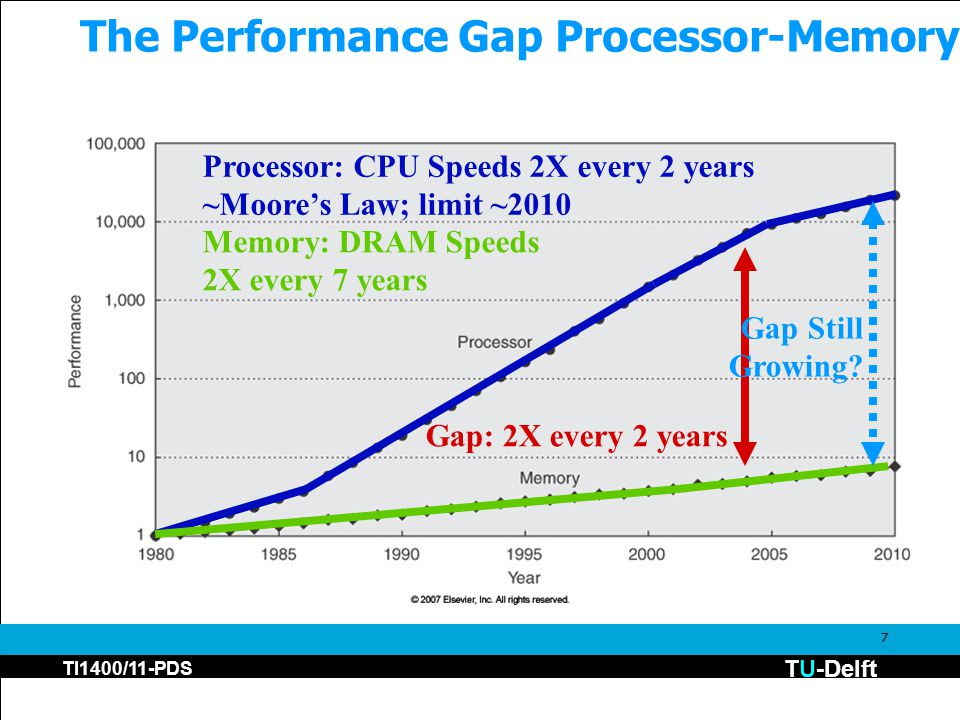
\includegraphics[width=0.8\textwidth]{img/slide_7.jpg}
  \end{figure}
  \vspace{0.5cm}

\end{itemize}

\end{document}
